% Metódy inžinierskej práce - semestrálny projekt Marek Čederle, AIS ID: 121193

\documentclass[10pt,oneside,slovak,a4paper]{article}

\usepackage[slovak]{babel}
%\usepackage[T1]{fontenc}
\usepackage[IL2]{fontenc} % lepšia sadzba písmena Ľ než v T1
\usepackage{graphicx}
\usepackage[utf8]{inputenc}
\usepackage{graphicx}
\usepackage{cite}
%\usepackage{pdfpages}
\usepackage{url} % príkaz \url na formátovanie URL
\usepackage{hyperref} % odkazy v texte budú aktívne (pri niektorých triedach dokumentov spôsobuje posun textu)
\usepackage[normalem]{ulem}
\useunder{\uline}{\ul}{}
\usepackage{float}
%\usepackage{times}

\pagestyle{headings}

\title{Vplyv umelej inteligencie na šach\thanks{Semestrálny projekt v predmete Metódy inžinierskej práce, ak. rok 2022/23, vedenie: Ing. Igor Stupavský }}

\author{Marek Čederle\\[2pt]
	{\small Slovenská technická univerzita v Bratislave}\\
	{\small Fakulta informatiky a informačných technológií}\\
	{\small \texttt{xcederlem@stuba.sk}}
	}

\date{\small 6. november 2022}



\begin{document}

\maketitle

\vspace*{\fill}

\begin{abstract}
 Počas pandémie COVID-19 a po vydaní seriálu Queen‘s Gambit (Dámsky gambit) z produkcie spoločnosti Netflix vypukol šachový boom v online, ale aj v reálnom svete. Po zrušení takzvaných OTB (Over the board) turnajov sa väčšina preniesla do online prostredia. V online prostredí číhajú nástrahy jednoduchého podvádzania pomocou umelej inteligencie (AI), respektíve takzvaných šachových botov. V tomto článku si rozoberieme, prečo a ako umelá inteligencia posúva hranice samotného šachu, ale aj jeho temnejšej strany a to podvádzania. Spomenieme si ako prvý raz umelá inteligencia vyhrala nad človekom a prečo to bol veľmi dôležitý krok ku zlepšeniu šachu ako takého. Na záver sa budeme venovať nedávnej šachovej dráme z turnaja Sinquefield Cup, ktorý sa odohral v St. Louis.
\end{abstract}

\vspace*{\fill}
\pagebreak


\section{Úvod}

Ľudstvo sa šachu venuje už stáročia, jeho korene siahajú až do roku 500 pred n. l.. Vzhľadom na množstvo ľudí, ktorí ho hrajú, sa v priebehu rokov menili aj jeho pravidlá a formy. Dnes sa šach nehrá len na drevenej šachovnici s ručne vyrobenými figúrkami. S príchodom digitalizácie sa šach dostal na  obrazovky počítačov ako aj superpočítačov.

Väčšina šachových podujatí, ktoré sa mali konať po začiatku pandémie sa preniesla do online sveta. Množstvo národných a medzinárodných turnajov sa hralo po prvý raz v histórii online. Počas pandémie sa šach stal jedným z mála športov, ktoré sa udržali. Veľké množstvo šachových veľmajstrov začalo s online prenosmi na platforme Twitch. Šach sa tam stal veľmi populárny a s vysielaním začalo aj veľa iných šachistov. S touto zmenou však  prišli pochybnosti o zručnostiach niektorých hráčov a prvé podozrenia z podvádzania.



\section{Ako funguje umelá inteligencia v šachu}

Keď pozorujeme vývoj umelej inteligencie\footnote{ang. AI - Artificial Intelligence} a šachu, musíme poznať, ako funguje a aké sú jej korene, aby sme lepšie pochopili možný vplyv umelej inteligencie na budúcnosť šachu.

Umelá inteligencia využíva v superpočítačoch techniky, ktoré jej pomáhajú vypočítať ideálny ďalší ťah. Pomocou problému hľadania stromu\footnote{ang. Tree Search Problem}, umelá inteligencia zvažuje aktuálne pozície šachových figúrok na šachovnici. Algoritmus následne udáva ďalší súbor inštrukcií na vykonanie.

Ak by umelá inteligencia používala iba jednoduchý brute force, aby vyskúšala všetky možné pozície (vrátane ilegálnych ťahov), tak už pri 13 figúrkach by sme vyčerpali všetko úložište dostupné na zemi aby sme vôbec tieto dáta uložili, kedže v šachu existuje asi $2^{111}$ až $2^{123}$ možností čo je viacej ako počet atómov v pozorovatelnom vesmíre.

V dôsledku toho môžeme povedať, že umelá inteligencia použije vyššie opísaný algoritmus a identifikuje všetky možné ťahy, ktoré môžu hráči vykonať. Umelá inteligencia má aj funkciu vyhodnocovania, ktorá presne určuje, aký dobrý je daný ťah. Týmto spôsobom pôjde iba do určitej hĺbky a nebude skúšať všetky možné kombinácie.

Vďaka tejto hodnotiacej funkcii môže umelá inteligencia preskúmať akékoľvek usporiadanie hracej plochy a vylúčiť ilegálne ťahy. Tým pádom sa znížia šance súpera na výhru.

Vytvoriť umelú inteligenciu, ktorá má za úlohu hrať šach však nie je jednoduché. Algoritmus stromov je síce zložitý, ale postupne už odborníci prekladajú logické inštrukcie na väčšinu šachových engine-ov\footnote{počítačový program, ktorý analyzuje šachovú pozíciu a generuje ťah alebo zoznam ťahov, ktoré považuje za najsilnejšie} aby vytvorili vylepšené neurónové siete.

\vspace*{\fill}

\section{Diagram práce na článku}
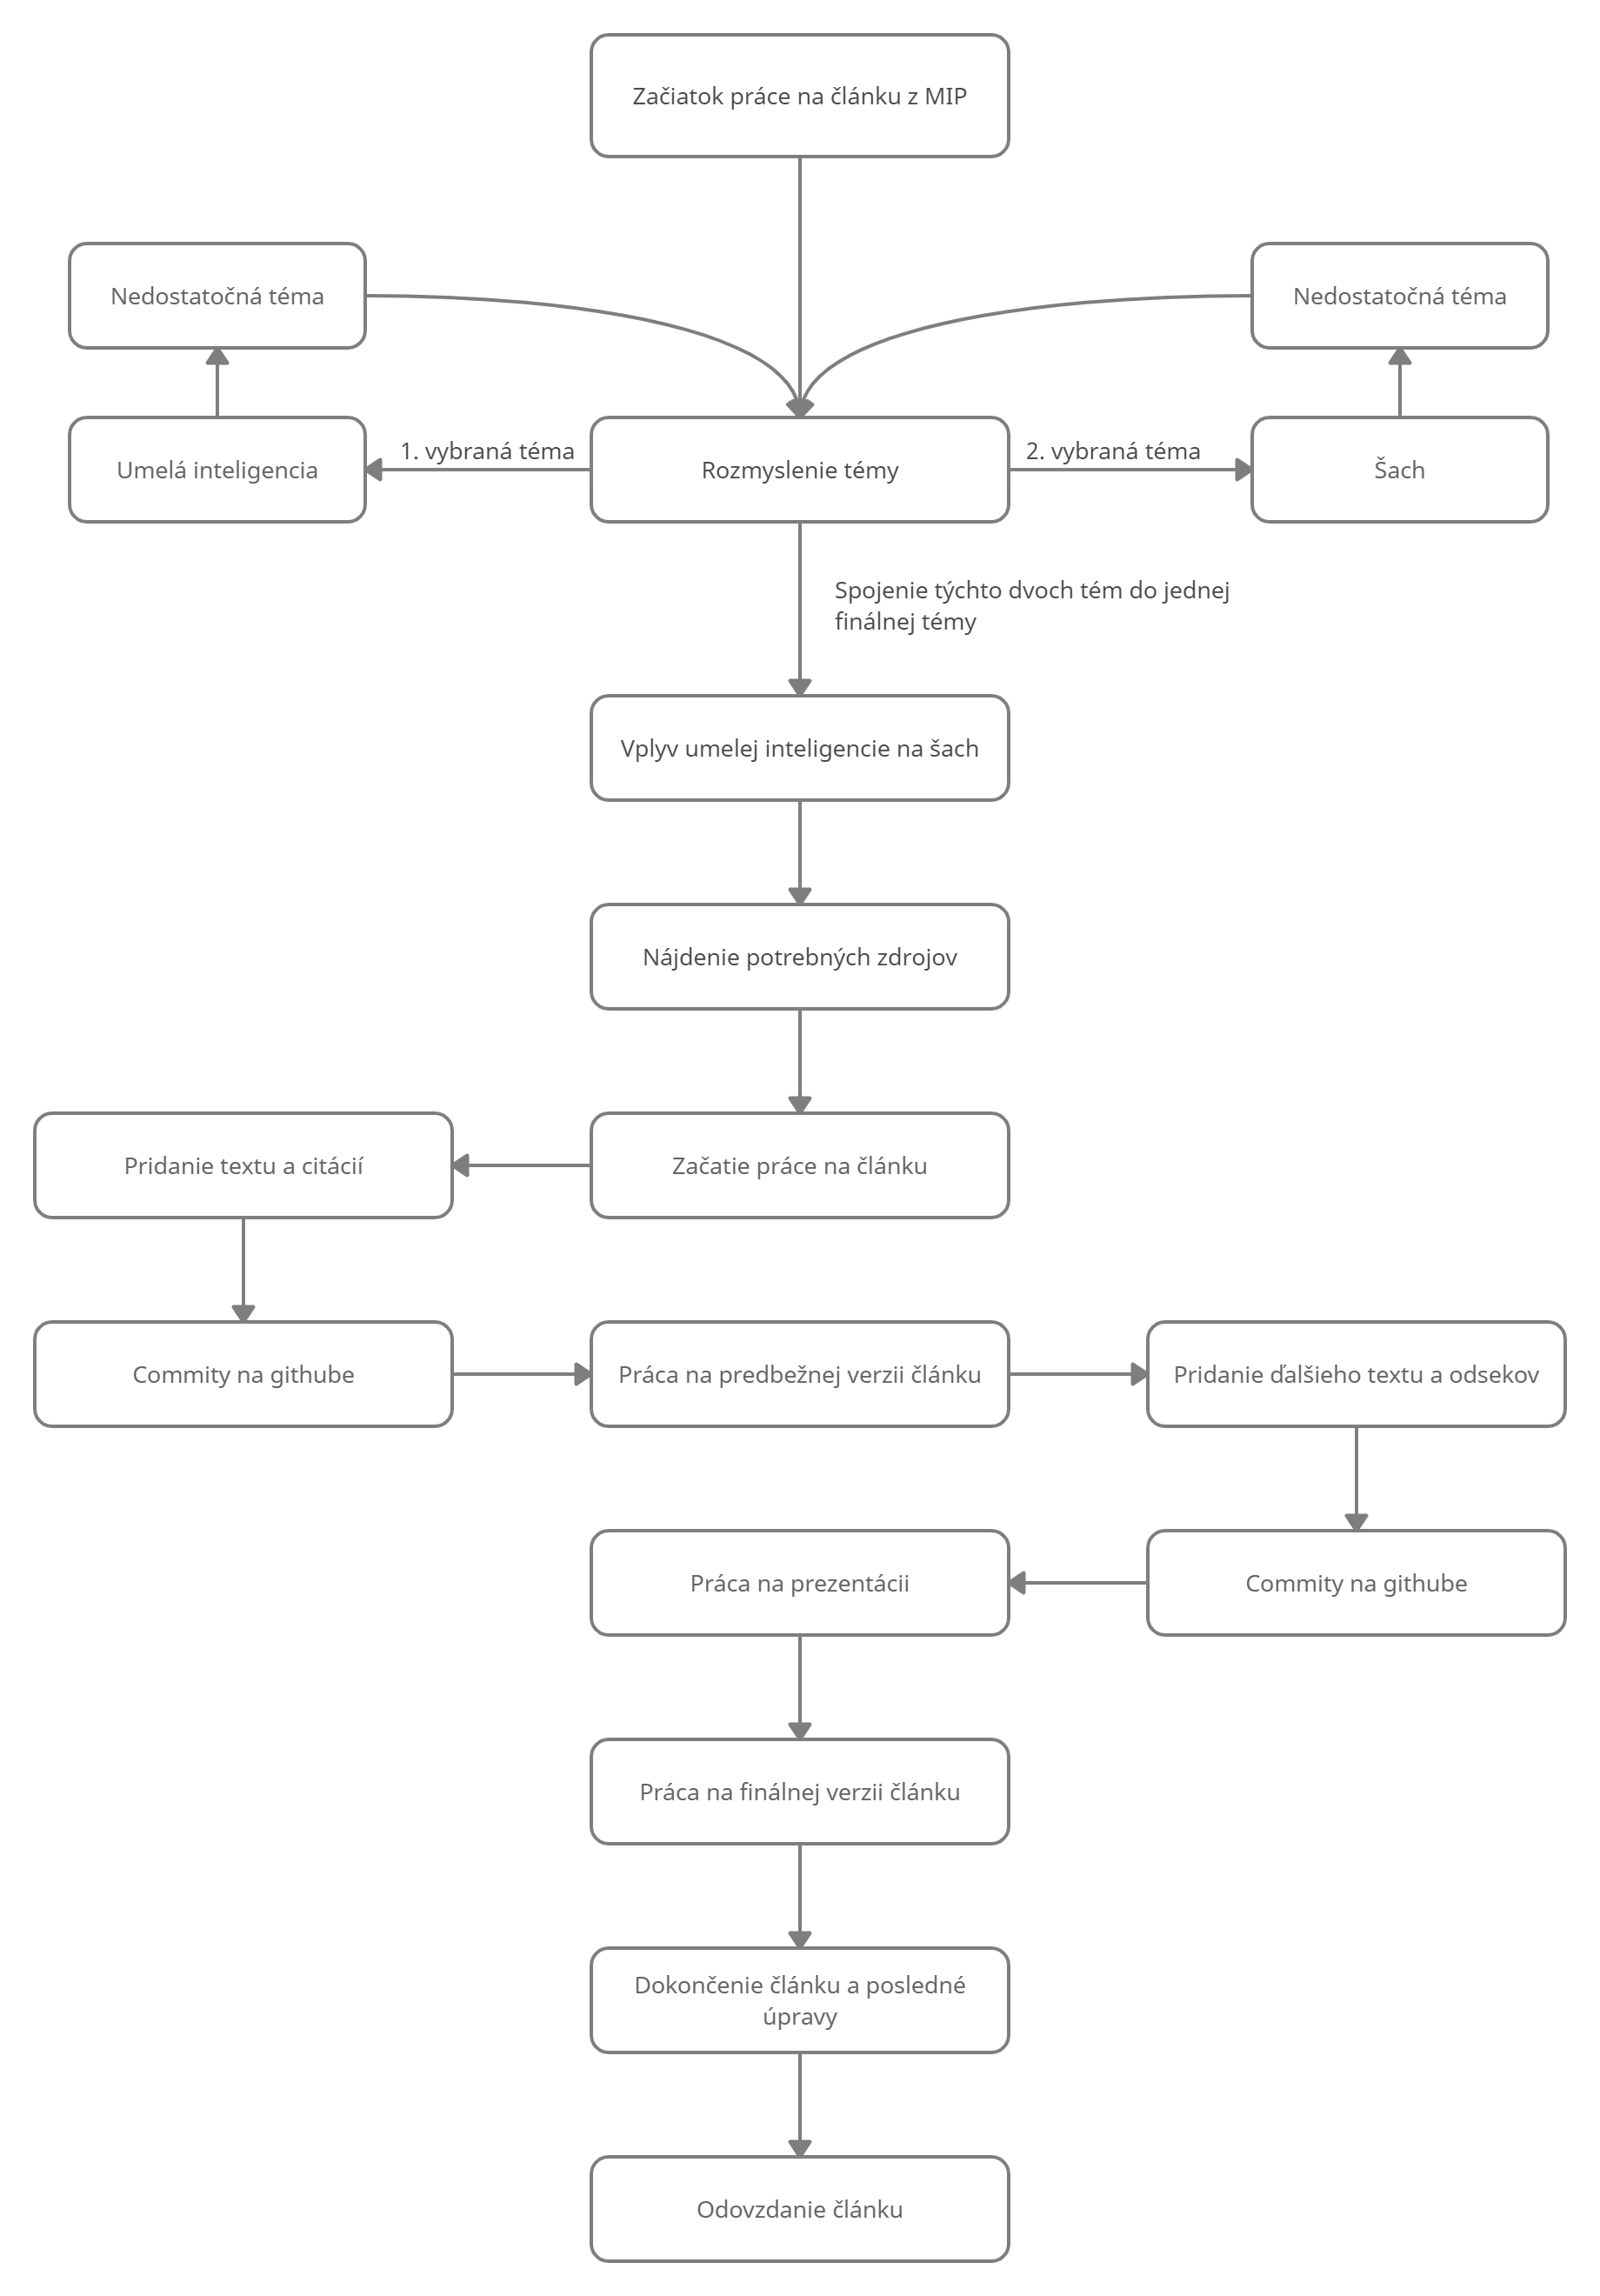
\includegraphics[scale=0.21]{diagram.jpg}

\section{Pokrok umelej inteligencie vo svete šachu}

Umelá inteligencia prechádza revolúciou, ale zároveň spôsobila revolučné zmeny v celom svete. Šach je jedna z mála oblastí, ktorá inšpiruje pokrok umelej inteligencie. Vývoj umelej inteligencie pre šach pokročil nad rámec hier a zmenil spôsob spolužitia strojov a ľudí. Pokrok umelej inteligencie, zvýraznený strategickými hrami, ovplyvnil mnohé ďalšie oblasti.

Jednou z najznámejších udalostí v boji človeka proti stroju bolo víťazstvo šachového enginu Deep Blue od spoločnosti IBM v roku 1997 proti slávnemu šachovému veľmajstrovi Garrymu Kasparovovi. Toto víťazstvo však bolo dosiahnuté najmä hrubou silou, keďže program Deep Blue prehľadával milióny pozícií za sekundu, aby mohol hrať šachy s o niečo vyššou silou (program vyhral zápas na 6 partií s rozdielom iba jedného bodu), takže asi viac zapôsobilo, že Kasparov s využitím ľudskej intuície dokázal byť stále takmer rovnako silný ako počítač prehľadávajúci milióny pozícií za sekundu. V nasledujúcich rokoch sa výpočtový výkon posunul do takej miery, že ani najlepší šachisti nemajú šancu poraziť moderný šachový engine.\cite{IM20}

Významný pokrok však nastal až o 2 desaťročia neskôr, keď nový šachový engine AlphaZero v roku 2017 vyhral zápas proti FOSS\footnote{ang. Free and Open Source Software - zadarmo, voľne šíriteľný s voľne prístupným zdrojovým kódom} enginu s názvom Stockfish, jednému z najvýkonnejších šachových enginov, aký bol kedy vytvorený, po procese samoučenia z daných dát trvajúcom len 4 hodiny.

Algoritmus AlphaZero sa nesnažil využiť hrubú silu na identifikáciu čo najväčšieho počtu ťahov na šachovnici. Namiesto toho napodobnil proces učenia sa človeka tým, že študoval veľký počtet šachových partií. Tvorcovia AlphaZero tvrdia, že algoritmus sa dokáže naučiť optimalizovať rozhodnutia v akomkoľvek scenári bez zmien alebo usmerňovania, a to bol skutočne prelom.\cite{IM20}

Daľší pokrok nastal, keď 19. novembra 2019 spoločnosť DeepMind predstavila ešte lepší algoritmus založený na spätnoväzobnom učení s názvom MuZero. Tento algoritmus sa naučil hrať šach lepšie ako AlphaZero aj bez toho aby mu niekto na začiatok povedal pravidlá hry.

Učiaci sa algoritmus MuZero má vo vyrovnávacej pamäti uložených maximálne 1 milión šachových partií, pričom paralelne sa hrá 3 000 partií.\cite{IM20} Bolo to možné vďaka tomu, že spoločnosť DeepMind mala prístup k rozsiahlej cloudovej infraštruktúre spoločnosti Google a používala tisíce Tensor\footnote{Novo predstavený čip, ktorý spoločnosť Google používa aj vo svojích mobilných telefónoch aby poháňal funckie spojené s umelou inteligenciou} čipov s procesorovými jednotkami špeciálne navrhnutými na výpočty neurónových sietí.

Neskôr sa aj open-source enginom, ako napríklad Leela Chess Zero, podarilo dosiahnuť úroveň MuZero a dokonca ju prekonať. Bolo to možné vďaka výpočtovému výkonu a vylepšeniam zdrojového kódu, ktoré poskytlo veľké množstvo dobrovoľníkov z celého sveta.

\vspace*{\fill}

\section{Systém hodnotenia v šachu}
Svetová šachová federácia (FIDE) udeľuje niekoľko titulov šachistom na základe ich výkonnosti a úrovne zručností. Tieto tituly, medzi ktoré patrí Veľmajster (GM), Medzinárodný majster a majster FIDE, sú medzi šachistami vysoko cenené, pretože sú uznaním ich schopností a môžu zlepšiť ich reputáciu a viditeľnosť v šachovom svete. Aby hráči získali titul FIDE, musia splniť určité kritériá a potom sa zúčastniť turnaja, kde ich výkon hodnotí porota. Kritériá pre každý titul sa líšia, ale vo všeobecnosti zahŕňajú faktory, ako je hodnotenie hráča, počet odohraných hier a ich výsledky v predchádzajúcich turnajoch. Tituly FIDE sa považujú za prestížne a môžu zlepšiť postavenie hráča v šachovej komunite.

Nasledujúca tabuľka\cite{FIDE} hovorí o tom koľko ľudí v šúčasnosti drží nejaký šachový titul:


\begin{table}[H]
		\def\arraystretch{1.5}
		\centering
		\begin{tabular}{|lccc|}
			\hline
			\multicolumn{4}{|c|}{Šachové tituly ("mužské"), November 2021}                                                     \\ \hline
			\multicolumn{1}{|l|}{Titul}                       & \multicolumn{1}{c|}{Muži}  & \multicolumn{1}{c|}{Ženy} & Spolu \\ \hline
			\multicolumn{1}{|l|}{Veľmajster (GM)}             & \multicolumn{1}{c|}{1700}  & \multicolumn{1}{c|}{39}   & 1739  \\ \hline
			\multicolumn{1}{|l|}{Medzinárodný   majster (IM)} & \multicolumn{1}{c|}{3782}  & \multicolumn{1}{c|}{126}  & 3908  \\ \hline
			\multicolumn{1}{|l|}{Majster FIDE   (FM)}         & \multicolumn{1}{c|}{8321}  & \multicolumn{1}{c|}{41}   & 8362  \\ \hline
			\multicolumn{1}{|l|}{Kandidátsky   majster (CM)}  & \multicolumn{1}{c|}{1964}  & \multicolumn{1}{c|}{22}   & 1986  \\ \hline
			\multicolumn{1}{|l|}{Spolu}                       & \multicolumn{1}{c|}{15767} & \multicolumn{1}{c|}{228}  & 15995 \\ \hline
		\end{tabular}
\end{table}

\section{Odhaľovanie podvodov na šachových\\
	 turnajoch pomocou AI}

Používanie AI na detekciu podvodov v šachových turnajoch má potenciál zlepšiť spravodlivosť a integritu hry. Systémy založené na AI dokážu analyzovať pohyby a správanie hráčov, aby identifikovali potenciálne prípady podvádzania napríklad používanie šachových enginov počas hry.

Jednou z potenciálnych výhod používania AI na detekciu podvodov na šachových turnajoch je to, že môže pomôcť zabezpečiť, aby sa hra hrala spravodlivo a podľa pravidiel. Analýzou pohybov a správania hráčov dokáže AI identifikovať potenciálne prípady podvádzania, ktoré si ľudskí rozhodcovia nemusia všimnúť. To môže pomôcť zabrániť hráčom, ktorí podvádzajú, získať nespravodlivú výhodu nad svojimi súpermi.

Ďalšou potenciálnou výhodou používania AI na detekciu podvodov v šachu je to, že môže pomôcť znížiť pracovné zaťaženie ľudských rozhodcov, ktorí by inak museli pozorne sledovať hráčov a priebeh partie, či hráči náhodou nevykazujú známky podvádzania. V tomto prípade umelá inteligencia odbremenila ľudí aj keď sa na ňu nemôžeme na 100\% spoľahnúť. Tým pádom sa môžu rozhodcovia zameriavať na iné problémy, ktoré môžu nastať.

\section{Problémy s detekciou podvodov}

Existuje niekoľko problémov s odhaľovaním podvádzania v šachu. Po prvé, môže byť ťažké určiť, či je konkrétny ťah výsledkom podvádzania alebo jednoducho chyby alebo kreatívnej a neočakávanej hry súpera. Po druhé, podvádzanie môže mať mnoho podôb, ako napríklad používanie šachového enginu alebo pomoc niekoho iného mimo hry, a odhaliť tieto činnosti môže byť náročné. Napokon, implementácia účinných opatrení na detekciu podvodov môže byť náročná bez toho, aby sa na hráčov uvalili obmedzenia, ktoré môžu brániť ich schopnosti hrať slobodne a spravodlivo.

Za zmienku tiež stojí, že v prvom rade môže existovať nedostatok konsenzu o tom, čo predstavuje podvádzanie. Rôzne šachové organizácie a turnaje môžu mať rôzne pravidlá a zásady týkajúce sa toho, čo je povolené a čo sa považuje za podvádzanie, čo môže sťažiť presadzovanie konzistentných noriem. Okrem toho používanie pokročilých technológií, ako sú počítačové programy, ktoré dokážu analyzovať a vyhodnocovať pozície, uľahčilo hráčom podvádzanie a pre funkcionárov je ťažšie to odhaliť.


\section{Nedávna šachová dráma}

Ak sledujete šachový svet, tak ste museli zachytiť nedávnu šachovú drámu spojenú so svetovým šampiónom v šachu, nórom Magnusom Carlsenom. Na turnaji Sinquefield Cup, ktorý sa odohral v St. Louis mladý šachista Hans Niemann porazil svetového šampióna Magnusa Carlsena. Na tom že nejaký veľmajster porazí iného nič nie je. Išlo o to, ako Niemann hral oproti Carlsenovi.

Niektorý hráči mali podozrenia že Niemann na turnaji podvádza. Carlsenova prehra nakoniec vyústila v to že odstúpil z turnaja a obvinil Niemanna z podvádzania. Následne Niemann priznal že podvádzal ale len dva krát v živote a to online keď mal 12 a 16 rokov. O dva týždne od incidentu sa zasa stretli pri šachovnici no tentokrát virtuálnej. Bol to online turnaj Julius Baer Generation Cup, kde Carlsen sa na protest vzdal po svojom prvom ťahu a ihneď vypol webkameru a odišiel. Z Carlsenovej strany okolo veci bolo ticho. Asi o mesiac v jeho oficiálnom stanovisku, ktoré zverejnil na svojom profile na Twitteri povedal: „Domnievam sa, že Niemann podvádzal viac a viac v poslednej dobe, ako verejne priznal.“\cite{TWI} Odmietol s ním hrať a apeloval na FIDE aby sprísnila už tak dosť prísne kontroly na podvádzanie.

Uplynul nejaký čas a Niemann podal na Carlsena, stránku Chess.com (ktorá mu zablokovalo prístup z podozrení na podvádzanie) a šachistu Hikarua Nakamuru žalobu z dôvodu očiernenia jeho mena, zničenia kariéri ale aj jeho života. Požaduje náhradu škody 150 miliónov dolárov. Bohužial je to veľmi smutné pre šachovú komunitu, že sa niečo takéto udialo. Výsledok žaloby budeme vedieť asi v priebehu niekoľkých mesiacov. Neostáva nám už nič iné iba čakať.


\section{Záver}

Na záver možno povedať, že vplyv umelej inteligencie na svet šachu bol významný. S rozvojom výkonných počítačových programov a algoritmov sú teraz šachisti schopní analyzovať a vyhodnocovať pozície a variácie na úrovni, ktorá bola predtým nepredstaviteľná. To viedlo k posunu v spôsobe hrania šachu s väčším dôrazom na prípravu a kalkuláciu.

Vzostup AI v šachu však tiež vyvolal diskusiu a polemiku. Niektorí tvrdia, že zvýšené spoliehanie sa na počítače znížilo kreativitu a individualitu šachistov, zatiaľ čo iní veria, že AI priniesla do hry nové výzvy a príležitosti.

Napriek týmto obavám je jasné, že AI mala hlboký vplyv na svet šachu a bude v tom pokračovať aj v budúcnosti. Keďže technológia neustále napreduje, bude zaujímavé sledovať, ako bude AI naďalej formovať spôsob, akým sa hrá šach a ako sa hráči prispôsobia týmto zmenám.

\section{Reakcia na prednášky}
\subsection{Inžinierska gramotnosť a informatika}

Na tejto prednáške som sa dozvedel zaujímavé informácie o tom, ako by sme ako inžinieri mali rozmýšlať, čo vôbec znamená byť inžinierom, čo je to informatika a čo nás bude tento semester čakať na tomto predmete.

Spomenuli sme si aj nástroj LaTeX. Príde mi to ako zaujímavý nástroj na tvorbu technickej dokumentácie avšak nie je zase jednoduchý takže som mu musel venovať nejaký ten čas.


\subsection{Inžinierska práca v informatike a písanie technického textu}

Na druhej prednáške sme si viacej vysvetlili a definovali kľúčové pojmy pre inžiniera a jeho prácu. Potom sme sa rozprávali na tému: Čo a ako sa učiť. Ja si osobne myslím že sa neviem dobre učiť kedže som nebol príliš motivovaný na strednej škole ale teraz na vysokej škole nemám príliš na výber takže sa učím.

Poslednú vec sme spomínali nástroj git a platfromu Github. Github mi príde nesmierne užitočný nástroj, často som ho používal aj používam v súvislosti s inštaláciou nejakých verejných skriptov alebo programov pre operačný systém Linux.

\subsection{Prezentácia: slajdy a prednes}

Siedma prenáška bola zameraná na prednes a prezentáciu pred publikom. Na začiatku sme si spomenuli nejaké pojmy a rozprávali sme sa ako (ne)prezentovať. Podstatené pre mňa bolo to, aby som mal počas môjho prezentovania jasnú štruktúru slajdov a nezasekával sa pri prejave.

Zhruba v strede prezentácie sme si spomenuli  nástroje na tvorbu prezentácií. Mne osobne vyhovuje pracovať na prezentáciách v programe MS Powerpoint takže aj svoju osobnú prezentáciu som robil v tomto programe. Prednášku by som zhodnotil ako celkom výdatnú.

\bibliography{literatura}
\bibliographystyle{alpha}
\end{document}